\chapter{Beschreibung der Software}

\section{Grundstruktur}

Die folgende Grafik illustriert das Grundsystem der Software.

\begin{figure}[h!]
		\centering
        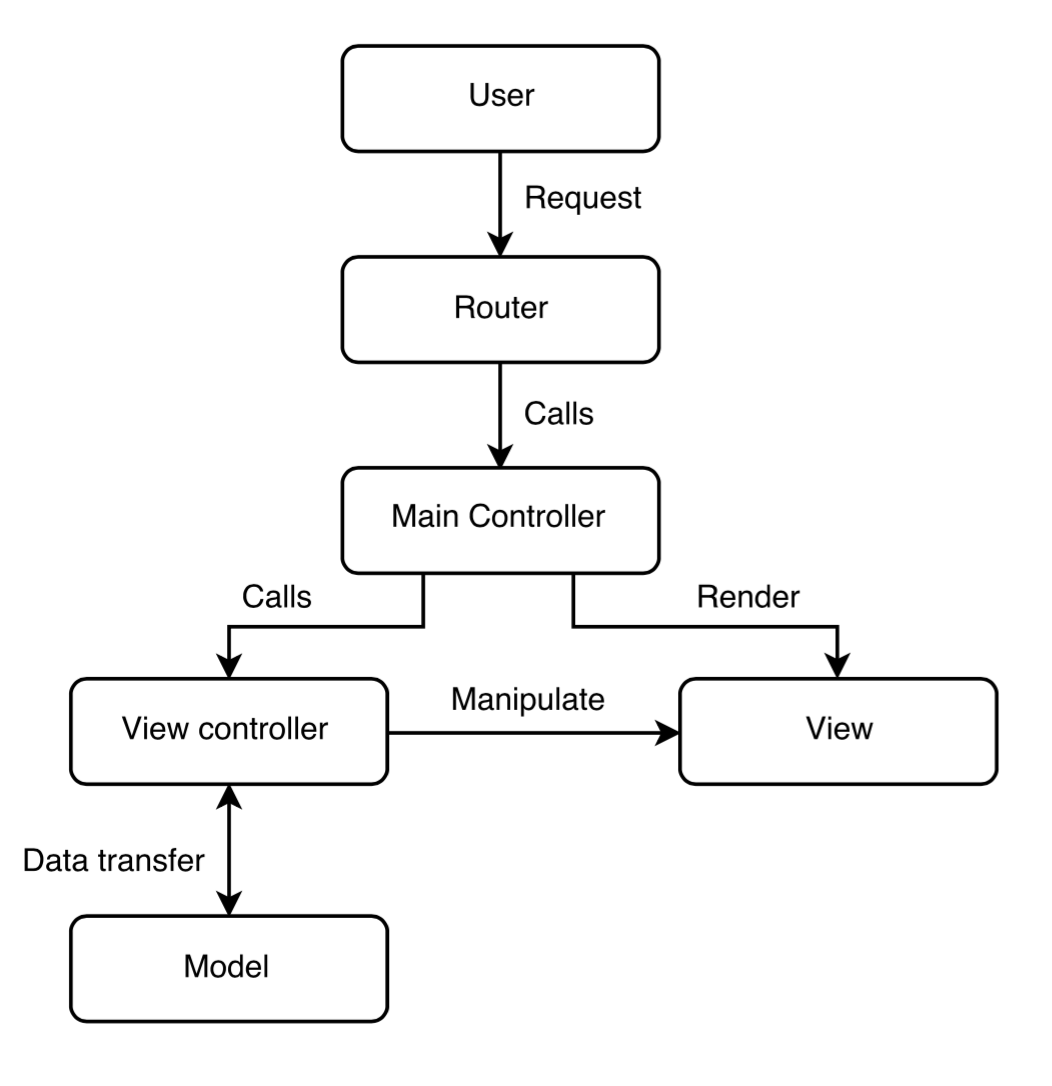
\includegraphics[width=0.7\textwidth]{./Includes/Software/architektur.png}
    \caption{Software Grundstruktur}
    \label{fig:somthing}
\end{figure}

Das Grundsystem ist nach dem MVC-Prinzip\footnote{MVC-Prinzip: Model View-Controller Abspaltung zur Strukturierung von Software} gestaltet.

\pm

Dabei ist das System aufgespalten in verschiedene Templates (Views),
die von ihrem zugehörigen Controller (View Controller) manipuliert 
werden. Der View Controller nutzt das Model um die nötigen Daten vom
Server zu erhalten.

\pm

Das Model ist (nach dem MVC-Prinzip) für die Datenhaltung zuständig.

\pm

\tb{Anmerkung:} Das komplette Grundsystem (Struktur, Core-Klassen) wurde von Steffen Lindner implementiert / entwickelt. 

\subsection{Router} 

Der Router wird genutzt, um ein URL-Template matching durchzuführen. 

\pm

Es lassen sich dadurch sehr leicht 'Pfade' entsprechenden Templates 
zuordnen. 

\begin{figure}[h!]
	\begin{lstlisting}[language=php]
Route::add("/home", function() {Controller::dispatch("home");});	
	\end{lstlisting}
	\caption{Beispielhafter Announce für eine Route}
\end{figure}

Dadurch sehen die URL's nicht nur schöner aus, es hat auch SEO\footnote{SEO: Suchmaschinennoptimierung} Vorteile.

\pm

Sobald die Route '/home' aufgerufen wird (beispielsweise: wolfgang.ne4y.de/home), wird die hinterlegte Funktion ausgeführt (in diesem Fall Controller::dispatch('home');)

\pm

Dabei wird über ein Patternmatching die aktuelle \tb{Requested-URI}
\footnote{Requested-URI: Angefragte URL Zeile, die vom Webserver an 
den PHP-Interpreter weitergegeben wird} mit den 'angekündigten' Pfaden verglichen. Stimmt ein Pfad überein, wird die hinterlegte Funktion ausgeführt.

\pm

Der Router nutzt außerdem einen Eintrag der Config-Klasse (siehe dazu Abschnitt zur Config-Klasse). Dort wird festgelegt, wie der Basepath aussieht. Liegt das System beispielsweise unter wolfgang.ne4y.de/meinDir/, so ist der Basepath meinDir. Dazu wird folgender Eintrag in einer Datei im config Ordner gesetzt: 

\begin{figure}[h!]
	\begin{lstlisting}[language=R]
	Config::set('basepath','meinDir');
	\end{lstlisting}
	\caption{Beispiel Basepath für die Router-Klasse}
\end{figure}

\subsection{Main Controller}

Der Main-Controller implementiert die grundlegenden Steuerfunktionen 
unserer Software. Dazu zählt das Rendern der Templates, das Aufrufen der entsprechenden Template-Controller sowie das Umleiten des Users.

\pm

Er gibt außerdem die Möglichkeit HTTP-Statuscodes an den Nutzer zurückzugeben.

\pm

Der Main Controller wird in den meisten Fällen direkt vom Router aufgerufen. Er implementiert folgende Methoden / Attribute:

\begin{figure}[h!]
		\centering
        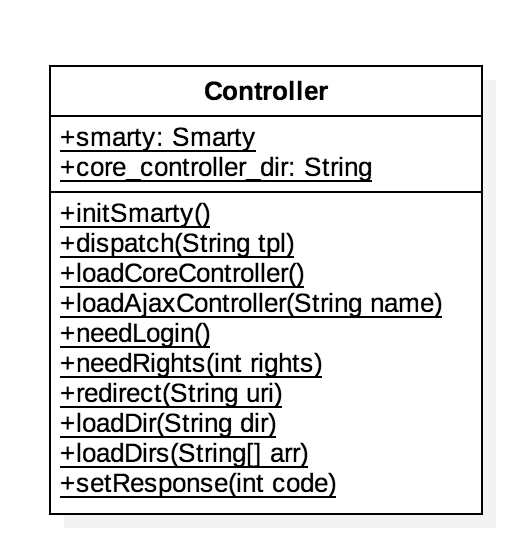
\includegraphics[width=0.6\textwidth]{./Includes/Software/Controller.png}
    \caption{Main-Controller}
\end{figure}

Dabei sind die wichtigsten Funktionen das Initialisieren eines Smarty Objects (initSmarty()), sowie das Dispatchen eines Templates (dispatch(String tpl), wird vom Router aufgerufen). Er hält auch das Smarty-Objekt gespeichert, über das die Variablen für die Templates gesetzt werden.

\begin{figure}[h!]
	\centering
	\begin{lstlisting}[language=php]
	Controller::$smarty->assign("myVar", "Das ist meine Variable")	
	\end{lstlisting}
	\caption{Der Maincontroller dient dazu Smartyfunktionalität zu ntuzen}
\end{figure}


\pm

Während des Dispatchprozesses wird der zugehörige Templatecontroller geladen.

\subsection{View} 

Der View wird durch ein Templatingsystem umgesetzt. Dafür verwendet 
unsere Software die Templateengine Smarty\footnote{Smarty: Templatingengine, mehr 
Informationen auf: http://smarty.net}.

Smarty wird genutzt, um den HTML-Code von der Businesslogik zu trennen. 

\pm

Dabei wird eine spezielle Templatesprache genutzt, die einem stark 
vereinfachtem PHP nahe kommt. Damit soll gewährleistet werden, dass im Template keine Businesslogik implementiert wird, um die klare Abtrennung der View vom Controller zu gewährleisten.

\pm

Ein kleines Beispiel soll die Interaktion von Controller und View verdeutlichen:

\begin{figure}[h!]
	\centering
	\begin{lstlisting}[language=php]
	Controller::$smarty->assign("Author", "Steffen Lindner");	
	\end{lstlisting}

    \caption{Beispielcontroller}
 \end{figure}
 
\begin{figure}[h!]
	\centering
	\begin{lstlisting}[language=html]
	<p>Name des Autors: {$Author}</p>
	\end{lstlisting}

    \caption{Beispielview}
 \end{figure}
 
Dadurch wird die gesamte Logik in den Controller verlagert und im Template lediglich durch einen 'Platzhalter' ersetzt.

\pm

Smarty erlaubt auch einfache logische Konstrukte wie 

\begin{itemize}
	\item If / Else / Elseif
	\item For / While / Foreach
	\item Isset / Empty
\end{itemize}


und viele Weitere. 

\subsection{Model}

Die Models werden zur Datenhaltung genutzt. Da wir keinen direkten Datenbankzugriff haben, sondern lediglich über eine Rest-API mit dem Server kommunizieren führen die Model die meisten Rest-Calls aus. Das gewährleistet eine klarere Trennung des Codes nach dem MVC-Prinzip.

\pm

Dazu wurde eine seperate Rest-Klasse geschrieben, die die Kommunikation mit dem Server verwaltet (dazu mehr im speziellen Abschnitt).

\pm

Die Models implementieren nun lediglich die speziellen Rest-Aufrufe, sowie einfache Verwaltungsaufgaben.

\pm

Eine genauere Beschreibung der Models folgt in den späteren Abschnitten.

\subsection{Index-Datei}

Die Index-Datei (index.php) ist der zentrale Ausgangspunkt unserer Software.

\pm

Alle Anfragen die der User stellt werden durch eine .htaccess-Datei unter Apache bzw. einer speziellen nginx-Konfiguration an die Index-Datei weitergeleitet. Dort lädt zunächst der Main-Controller alle Klassen (Core- und 'normale' Klassen), sowie alle Models (dazu später mehr). In der Index-Datei werden außerdem alle Routen aus dem Routen-Ordner geladen (angegeben durch einen Eintrag in der Config-Datei, siehe dazu den Abschnitt zur Config-Klasse).

\pm

Schließlich wird dort der User initialisiert (es wird erkannt, ob der Nutzer eingeloggt ist, was für Rechte er hat usw.) und der Routingprozess gestartet (und somit das angefragte Template samt zugehörigem Controller geladen). 
\section{Core Klassen}

Unsere Software ist eingeteilt in 'normale' Klassen und Core Klassen. Die Core Klassen implementieren allgemeinere Funktionen, die von der gesamten Software genutzt werden.

\pm

Zu den Core Klassen gehören:

\begin{itemize}
	\item Notify Klasse
	\item Controller Klasse (Main Controller, bereits beschrieben)
	\item Config Klasse
	\item RestApi Klasse
	\item Route Klasse (bereits beschrieben)
\end{itemize}
	

So gut wie alle Core-Klassen sind statisch implementiert. Das heißt, es wird kein Objekt der einzelnen Klassen erzeugt. Das hat zum Einen den Grund, dass sie von der 'Logik' her keinen richtigen Zustand haben. Zum Andern ist es aus programmiertechnischer Sicht einfacher, bzw. praktischer, direkt auf die Funktionen zugreifen zu können, ohne auf ein Objekt angewiesen zu sein.

\pm

 Die Models hingegen sind objektorientiert implementiert, d.h. um sie richtig nutzen zu können müssen zunächst Objekte erstellt werden.

\pm

Einige der Core-Klassen sollen im Folgenden etwas näher beschrieben werden.

\subsection{Notify Klasse}

Die Notify Klasse wird genutzt, um Meldungen an den Nutzer auszugeben.

\begin{figure}[h!]
		\centering
        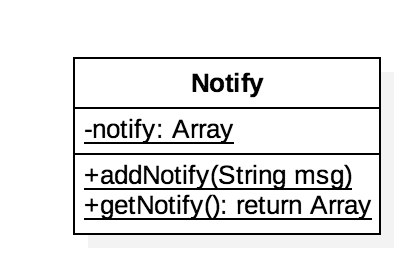
\includegraphics[width=0.3\textwidth]{./Includes/Software/Notify.png}
    \caption{Notify Klasse}
\end{figure}

Der Main-Controller liest nach dem Abarbeiten der View-Controller die erstellten Nachrichten aus und speichert sie in einer Smarty-Variable, die anschließend vom Template ausgegeben wird. Dadurch können die View-Controller unabhängig voneinander Nachrichten an den Nutzer zurückgeben, ohne sich selbst um die Darstellung kümmern zu müssen.

\subsection{Config Klasse}

Die Config Klasse wird genutzt, um Konstanten anzulegen, wie beispielsweise der Basepath des Systems, wie viele Kategorieren pro Seite angezeigt werden sollen o.ä.

\begin{figure}[h!]
		\centering
        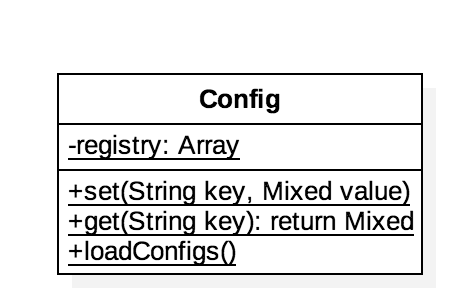
\includegraphics[width=0.5\textwidth]{./Includes/Software/Config.png}
    \caption{Config Klasse}
\end{figure}

Es handelt sich dabei um einen einfachen Key-Value Store. Aufgrund der schwachen Typisierung von PHP kann jede Art von Value gespeichert werden.

\newpage

\subsection{RestApi Klasse}

Da die gesamte Kommunikation mit dem Server über eine Rest-API\footnote{Rest: Representational State Transfer, Programmparadigma für verteile Systeme} abläuft, wurde eine zentrale Klasse geschrieben, die die Kommunikation mit dem Server erleichtern soll.

\pm

Die RestApi-Klasse implementiert dabei folgende Methoden:

\begin{figure}[H]
		\centering
        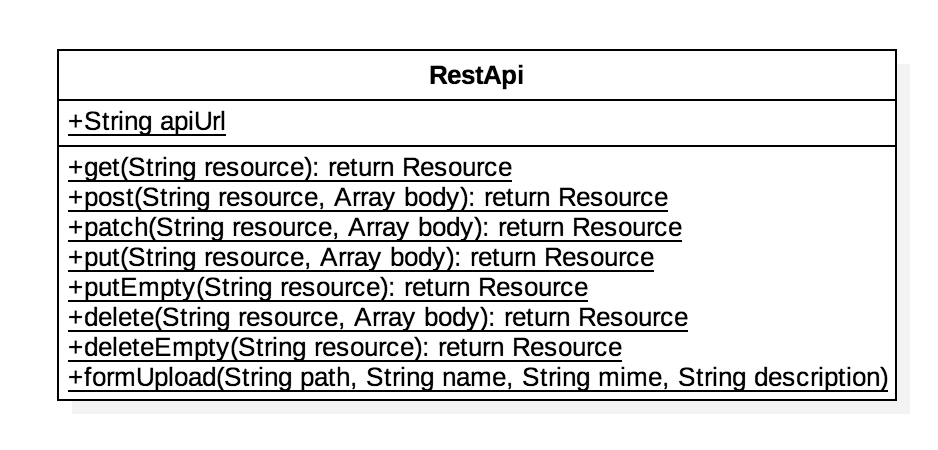
\includegraphics[width=0.8\textwidth]{./Includes/Software/RestApi.png}
    \caption{RestApi Klasse}
\end{figure}

Es können die grundlegenden HTTP-Requests get, post, patch, put, delete ausgeführt werden. Dafür wurde die PHP-Implementierung von cURL\footnote{cURL: CURL Url Request Library, Bibliothek zum Ausführen von HTTP-Requests} verwendet.

\pm

Beispielhafte Verwendung der RestApi-Klasse:

\begin{figure}[H]
	\begin{lstlisting}
Last login: Fri Jul  8 22:34:48 on ttys002
Steffen@Steffens-MBP:~/ownCloud/Projects/www/ProgrammierProjektSS16\:$ php -a
Interactive shell

php > include("model/User.php");
php > User::initUser();
php > include("libs/Core/RestApi.php");
php > var_dump(json_decode(RestApi::get("/videos?limit=1")));
object(stdClass)#2 (7) {
  ["total"]=>
  string(3) "132"
  ["items"]=>
  array(1) {
    [0]=>
    object(stdClass)#3 (11) {
      ["id"]=>
      string(1) "4"
     ...}
php > 
	\end{lstlisting}
	\caption{Beispielhafte Verwendung der RestApi-Klasse}
\end{figure}

(die Ausgabe wurde aus Platzgründen abgeschnitten).

\pm

Die RestApi-Klasse ist damit die Schnittstelle zwischen unserem System und dem zur Verfügung gestellten Backendsystem.

\section{Models}

\subsection{User}

Das User-Model verwaltet alle Daten des Users. Dazu zählt beispielsweise die UserID, die Rechte des Users, Name, Email etc.

\pm

Das User-Model implementiert folgende Funktionalitäten:

\begin{figure}[H]
		\centering
        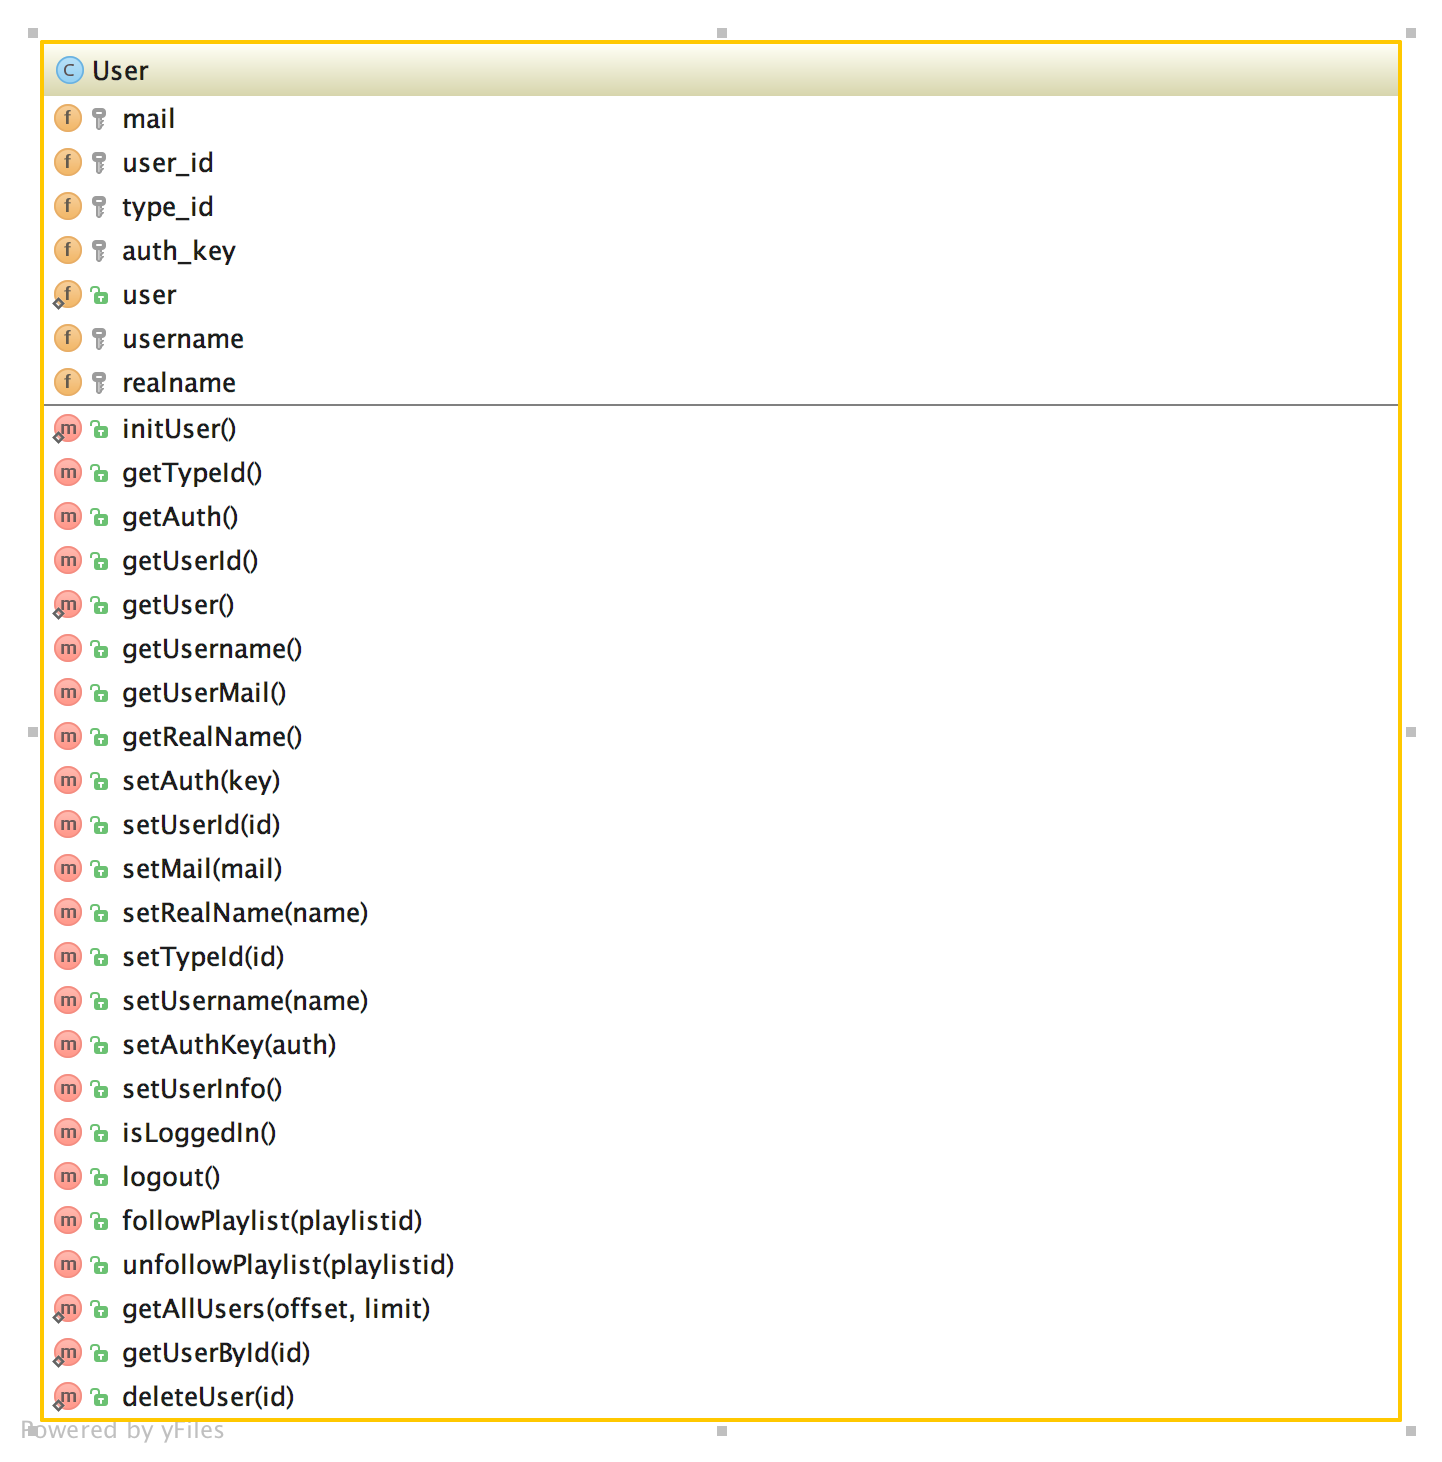
\includegraphics[width=0.9\textwidth]{./UML/User.png}
    \caption{User Model}
\end{figure}

Das User-Model ist aus programmiertechnischer Sicht eine Mischung aus statischer und objektorientierter Implementierung. Um das User Objekt nicht durch alle Seiten zu 'tragen' wird zunächst in der Index-Datei der User initiiert. Dabei wird ein neues (statisches) User Objekt erstellt und ggf. mit vorhandenen Daten (aus Sessions) initialisiert (notwendig, damit ein Nutzer eingeloggt bleibt und nicht bei jedem Seitenaufruf die Userdaten erneut vom Server abgefragt werden müssen).

\pm

Ab diesem Moment kann man in jedem Controller das aktuelle Userobjekt erhalten, um anschließend objektspezifische Operationen auszuführen.

\begin{figure}[H]
	\begin{lstlisting}
		User::getUser()->getUserMail();	
	\end{lstlisting}
	\caption{Beispielaufruf, um die Mail des aktuellen Benutzers zu erhalten}
\end{figure}

Innerhalb des User-Models sind die oben genannten Funktionalitäten implementiert, wobei die Kommunikation mit dem Backendsystem über die bereits beschriebene RestApi Klasse abläuft.

\pm

\tb{Anmerkun:} Das User-Model wurde größtenteils von Steffen Lindner implementiert.

\subsection{Kategorie}

Das Kategorien Model verwaltet die Daten für eine Kategorie bzw. allgemeine Funktionen die Kategorien betreffen. Dabei wurden alle Methoden, die nicht speziell einer Kategorie zugeordnet werden (wie beispielsweise das Suchen nach Kategorien bezüglich eines Namens) statisch implementiert. 

\pm

Aufgrund der unterschiedlichen Programmierer kommt es allerdings vor, dass Methoden, die eigentlich einer speziellen Kategorie zugeordnet werden können (wie beispielsweise das Hinzufügen eines Videos zu einer Kategorie) ebenfalls statisch implementiert wurden.

\pm

Das Kategorie-Model implementiert folgende Methoden:

\begin{figure}[H]
		\centering
        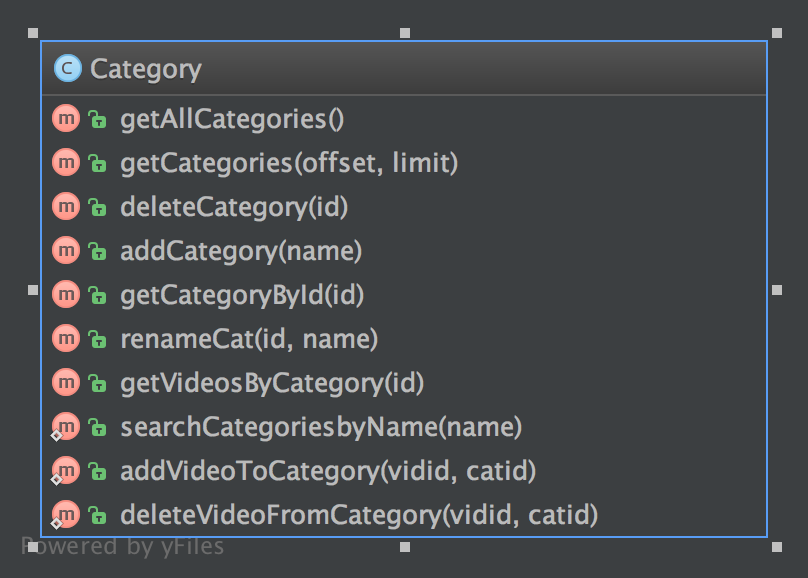
\includegraphics[width=0.7\textwidth]{./UML/Category.png}
    \caption{Kategorie Model}
\end{figure}

\tb{Anmerkung:} Das Kategorien-Model wurde (größtenteils) von Steffen Lindner (erster Teil) und Maximillian Pfister (zweiter Teil) implementiert.

\subsection{Video}
Das Video Model, enthält zum einen alle Metadaten eines Videos und zum anderen statische Methoden um auf eine bestimmte Anzahl Videos zuzugreifen, sowie Kommentare, Ratings und Videos hinzuzufügen.
\begin{figure}[h!]
\centering
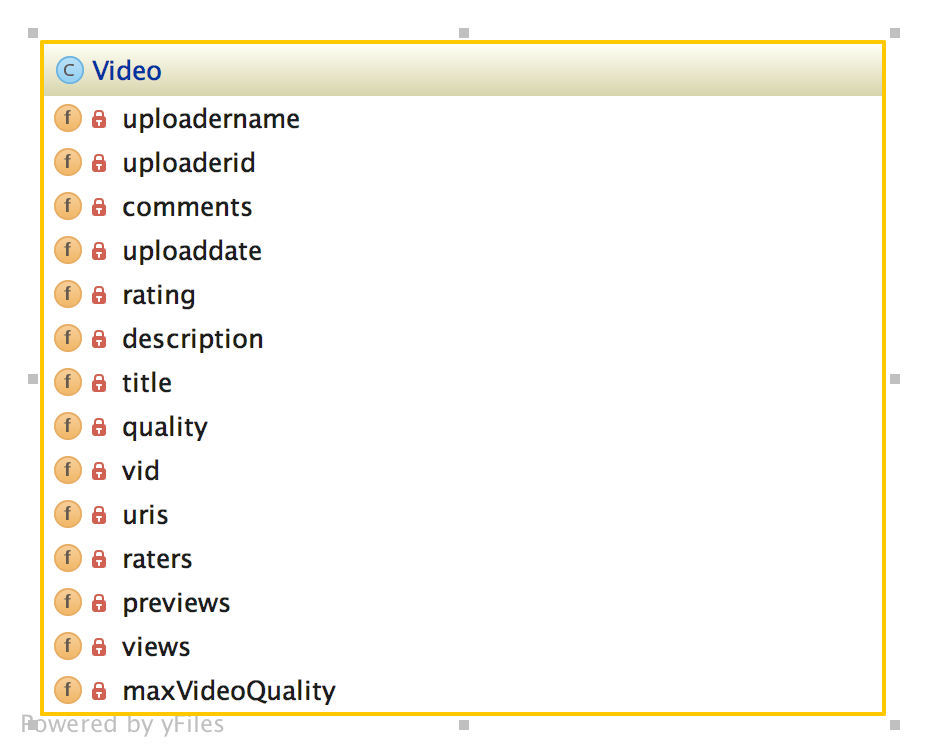
\includegraphics[width=0.7\textwidth]{./UML/VideoMeta.png}
\caption{Metadaten eines Videos}
\end{figure}
\clearpage
Beim erstellen eines Video Objektes durch übergeben einer ID wird durch den Konstruktor der Klasse automatisch alle Metadaten durch ein REST-Call gesetzt.
\begin{lstlisting}[language=php]
public function __construct($id){
            $ret = json_decode(RestAPI::get("/videos/".$id,array("id" => $id)));

            if (isset($ret->error)){
                Controller::redirect("/404");
            }
            else{
                $this->views = $ret->views;
                $this->vid = $ret->id;
                $this->title = (empty($ret->title) ? 'Kein Titel' : $ret->title);
                $this->description = $ret->description;
                $this->uploaderid = $ret->uploaderid;
                $this->uploadername = $ret->uploadername;
                $this->uploaddate = $ret->uploaddate;
                $this->rating = (empty($ret->rating) ? 0 : $ret->rating);
                $this->uris = $ret->uri;
                $this->previews = $ret->previews;
                $this->comments = $ret->comments;
                $this->raters = $ret->ratings->items;
                $this->maxVideoQuality = $ret->maxVideoQuality;
            }

        }
\end{lstlisting}
Das sind alle Metadaten die der Backend Server liefert. \pm
\begin{figure}[h!]
\centering
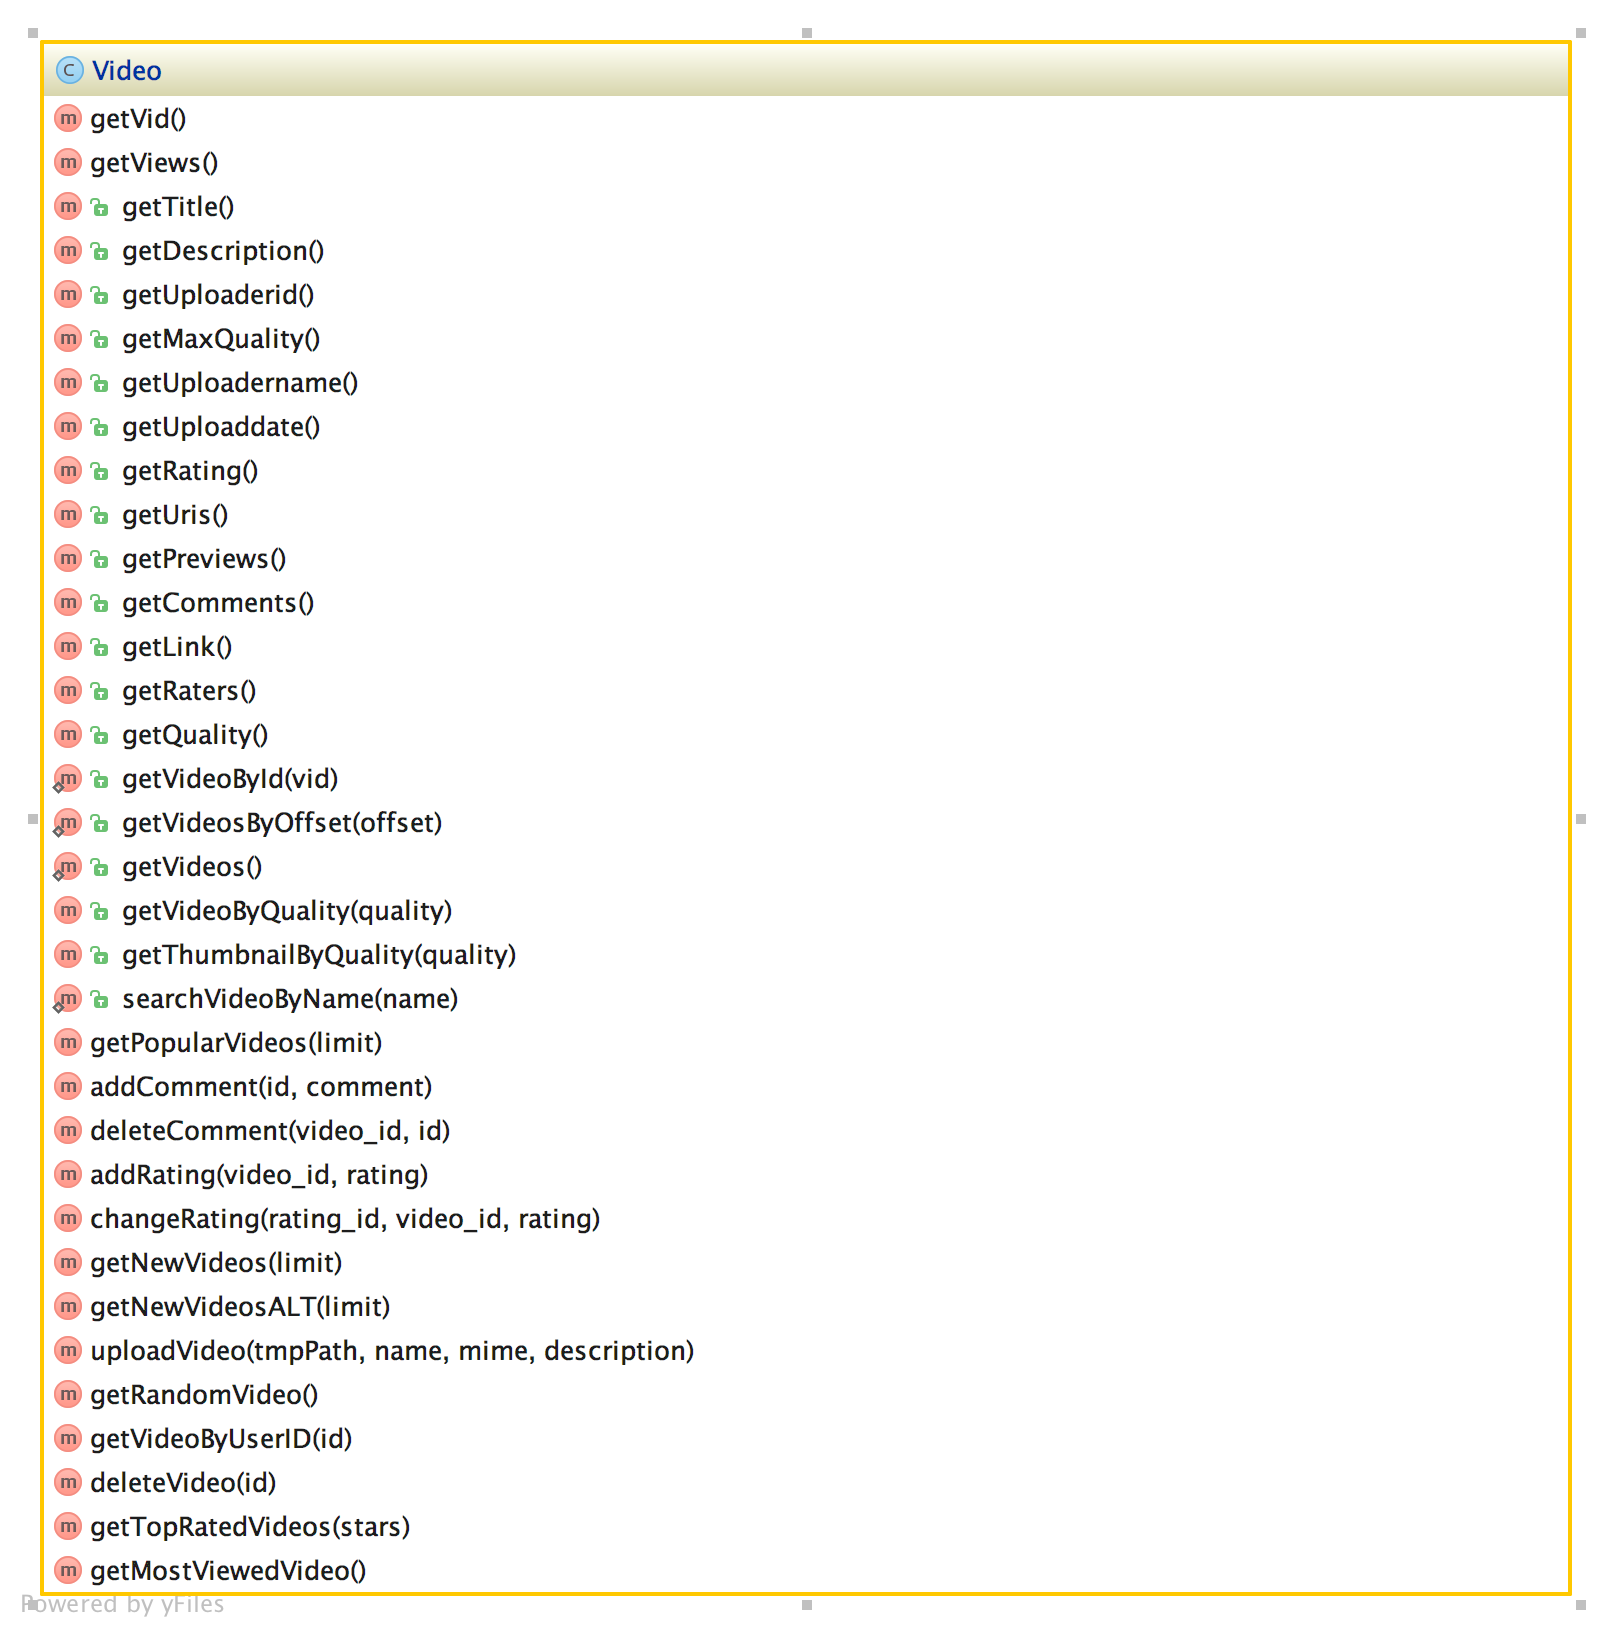
\includegraphics[width=0.7\textwidth]{./UML/VideoFunction.png}
\caption{Funktionen der Video Klasse}
\end{figure}
Neben den trivialen Getter Methoden wird in der Video Klasse noch Funktionalitäten rund um das Video als statische Methoden implementiert.\\
\texttt{getTopRatedVideos, getRandomVideo, getNewVideos, getVideoByUserID} und \texttt{getPopularVideos} geben durch gezielte Suche bestimmte Arten von Videos zurück.\\
\texttt{addComment,deleteComment,addRating, uploadVideo, deleteVideo, searchVideoByName} und \texttt{changeRating} stehen als Schnittstellen zwischen ihren jeweiligen AJAX Implementationen und dem Backend.\\
\begin{lstlisting}[language=php,caption=Examplarische Implementation einer Methode des Video Models]
public static function getPopularVideos($limit){
        $ret = RestAPI::get("/search?type=popularvideos&limit=" . $limit); //REST Call
        return json_decode($ret);//Als PHP JSON (stdClass) Objekt zurückgeben
	}
\end{lstlisting} 
\tb{Anmerkung:} Die Klassenstruktur und die nicht statischen Methoden wurden von Finn Ickler implementiert. Die statischen Methoden vom Rest des Teams.
\subsection{Playlist}

Das Playlist Model verwaltet die Daten für eine Playlist bzw. allgemeine Funktionen die Playlisten betreffen. Da die Funktionen, die Playlisten betreffen, auch in der Suchfunktion oder z.Bsp. in der Video Wiedergabe genutzt werden, wurden diese alle statisch implementiert.

\pm

Das Playlist-Model implementiert folgende Methoden:

\begin{figure}[H]
		\centering
        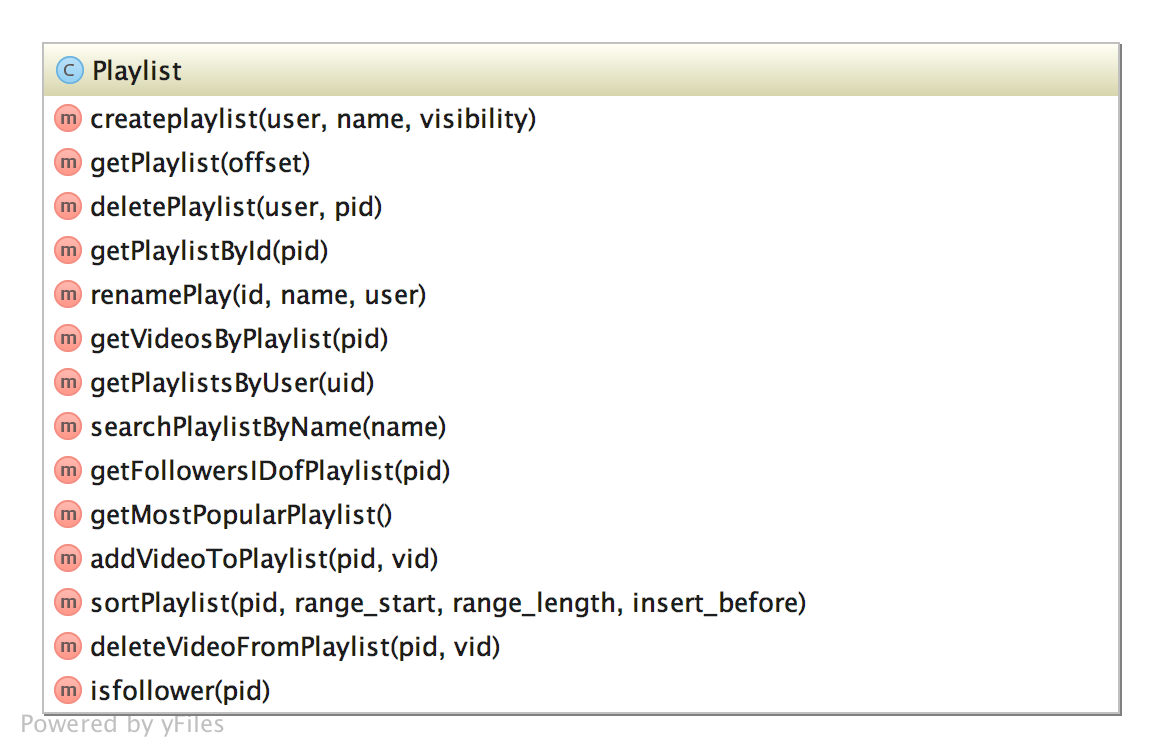
\includegraphics[width=0.7\textwidth]{./UML/Playlist.png}
    \caption{Kategorie Model}
\end{figure}

\tb{Anmerkung:} Das Playlist-Model wurde von Dominik Spoerle, Finn Ickler und Maximillian Pfister (zweiter Teil) implementiert.


\section{Umgesetzte Funktionalitäten}
Das System implementiert folgende Funktionalitäten:

\begin{itemize}
	\item Login (Steffen Lindner)
	\item Registrierung (Maximillian Pfister)
	\item Profil (ansehen / bearbeiten) (Steffen Lindner)
	\item Kategorienverwaltung (anzeigen, anlegen, bearbeiten) (Steffen Lindner)
	\item Playlistverwaltung (Dominik Spoerle)
	\item Playlistumsortierung (Steffen Lindner)
	\item Videosuche \& Ergebnisanzeige (Finn Ickler)
	\item Videoansicht (Finn Ickler)
	\item Videos kommentieren / bewerten (Steffen Lindner)
	\item Video upload (Finn Ickler)
	\item Neuste Videos / Favoriten (Dominik Spoerle)
	\item Playlist abonieren / deabonieren, Videos zu Kategorien hinzufügen / entfernen (Maximillian Pfister)
	\item Rechtemanagment (Steffen Lindner \& Finn Ickler)
\end{itemize}

\section{Verwendete Drittsoftware}
\begin{itemize}
	\item \href{http://www.smarty.net/}{Smarty PHP Template Engine}
	\item \href{https://jquery.com/}{JQuery}
	\item \href{http://getbootstrap.com/}{Bootstrap Framework}
	\item \href{https://robohash.org/}{RoboHash}
	\item \href{http://videojs.com/}{VideoJS}
	\item \href{https://github.com/RubaXa/Sortable}{sortable.js}
	\item \href{http://plugins.krajee.com/file-input}{fileinput.js}
\end{itemize}













